\documentclass[aspectratio=169,obeyspaces,spaces,hyphens,dvipsnames]{beamer}
\usepackage[utf8]{inputenc}
\usepackage{minted}
\usepackage{hyperref}

\mode<presentation>
\usetheme{FreeElectrons}

\def\signed #1{{\leavevmode\unskip\nobreak\hfil\penalty50\hskip2em
  \hbox{}\nobreak\hfil(#1)%
  \parfillskip=0pt \finalhyphendemerits=0 \endgraf}}

\newsavebox\mybox
\newenvironment{aquote}[1]
  {\savebox\mybox{#1}\begin{quotation}}
  {\signed{\usebox\mybox}\end{quotation}}

\title{Running UBI/UBIFS on MLC NAND}
\conference{Embedded Linux Conference 2016}
\authors{Boris Brezillon}
\email{boris@free-electrons.com}
\institute{Free Electrons}
\slidesurl{http://free-electrons.com/pub/conferences/2016/elc/brezillon-nand-framework}

\begin{document}

\addtocontents{toc}{\protect\setcounter{tocdepth}{-1}}
\section{Running UBI/UBIFS on MLC NAND}
\addtocontents{toc}{\protect\setcounter{tocdepth}{2}}

\subsection{MLC NANDs constraints: where the nightmare begins}

\begin{frame}{SLC NANDs: Finger in the nose}
  \begin{itemize}
  \item TODO: add an image (search on a tumblr?)
  \end{itemize}
\end{frame}

\begin{frame}{MLC NANDs: Ouch!}
  \begin{itemize}
  \item TODO: add an image (search on a tumblr)
  \end{itemize}
\end{frame}

\begin{frame}{MLC NAND constraints: What we knew}
  \begin{itemize}
  \item Reduced lifetime: limited number of P/E cycles (5000-10000).
  \item Pages within an erase block have to be programmed in ascending
	order.
  \item Data rentention issues: pretty much the same problem we see
	on SLC NANDs, but a different order of magnitude.
  \item Paired pages: why the hell did they decide to assign the same
	cell to different NAND pages?
  \item Unstable bits: you'd better make sure your board has enough
	power to finish the current erase or program operation, and
	prevent future operations from happening when you are about to
	experience a power-cut.
  \end{itemize}
\end{frame}

\begin{frame}{MLC NAND constraints: Reduced lifetime}
  \begin{itemize}
  \item Not a big problem: we just need to make sure we correctly
	distribute the wear over the NAND device.
  \item UBI is already taking care of that.
  \item May require some tweaking at the UBI level: the default values
	are not suitable for MLC NANDs.
  \end{itemize}
\end{frame}

\begin{frame}{MLC NAND constraints: Data retention issues (1)}
  \begin{itemize}
  \item A NAND cell can see its state changed (charge loss or gain):
	this is what we call bitflips.
  \item Two known sources:
    \begin{itemize}
    \item Read/write disturbance: reading/programming a cell can
	  change neighbour cells state
    \item Inherent charge loss: NAND cells tend to loose their
	  charge over-time. This is emphasized when NAND cells are
	  worn out.
    \end{itemize}
  \item Solutions:
    \begin{itemize}
    \item Increase the ECC strength: usually, this is NAND controller
	  dependent, and even with a strong ECC, you'll hit
	  uncorrectable errors at some point.
    \item Regularly read NAND eraseblocks to detect those that are
	  showing a lot of bitflips, and move the data somewhere else
	  before the ECC is unable to correct these errors.
    \end{itemize}
  \end{itemize}
\end{frame}

\begin{frame}{MLC NAND constraints: Data retention issues (2)}
  \begin{itemize}
  \item MLC cells expose 4 different states instead of 2 states for
	SLC cells.
  \item In MLC cells, distance between states are smaller: data
	retention issues are emphasized.
  \item The smaller the process the closer the cells are, which makes
	read/write disturbance worse.
  \end{itemize}
\end{frame}

\begin{frame}{MLC NAND constraints: Unstable bits}
  \begin{itemize}
  \item Problem described here
	\url{http://www.linux-mtd.infradead.org/doc/ubifs.html\#L_unstable_bits}
  \item Reported by some people on the MTD mailing list
  \item We did not see it during our experimentation
  \item NAND vendors do not communicate on this problem and each
	time we ask, they say they are not aware of this kind of
	problems.
  \item What is described as a black and white problem may actually
	be more subtle: interrupting a program or erase operation
	just before it finishes might leave the page/block in a 'valid'
	state but with a lot of bitflips.
  \item If this assumption turns out to be true, UBI should be able to
	detect that the number of bitflips is high and decide to move
	the data somewhere else or re-erase the block.
  \end{itemize}
\end{frame}

\begin{frame}{MLC NAND constraints: MLC cells}
  \begin{center}
    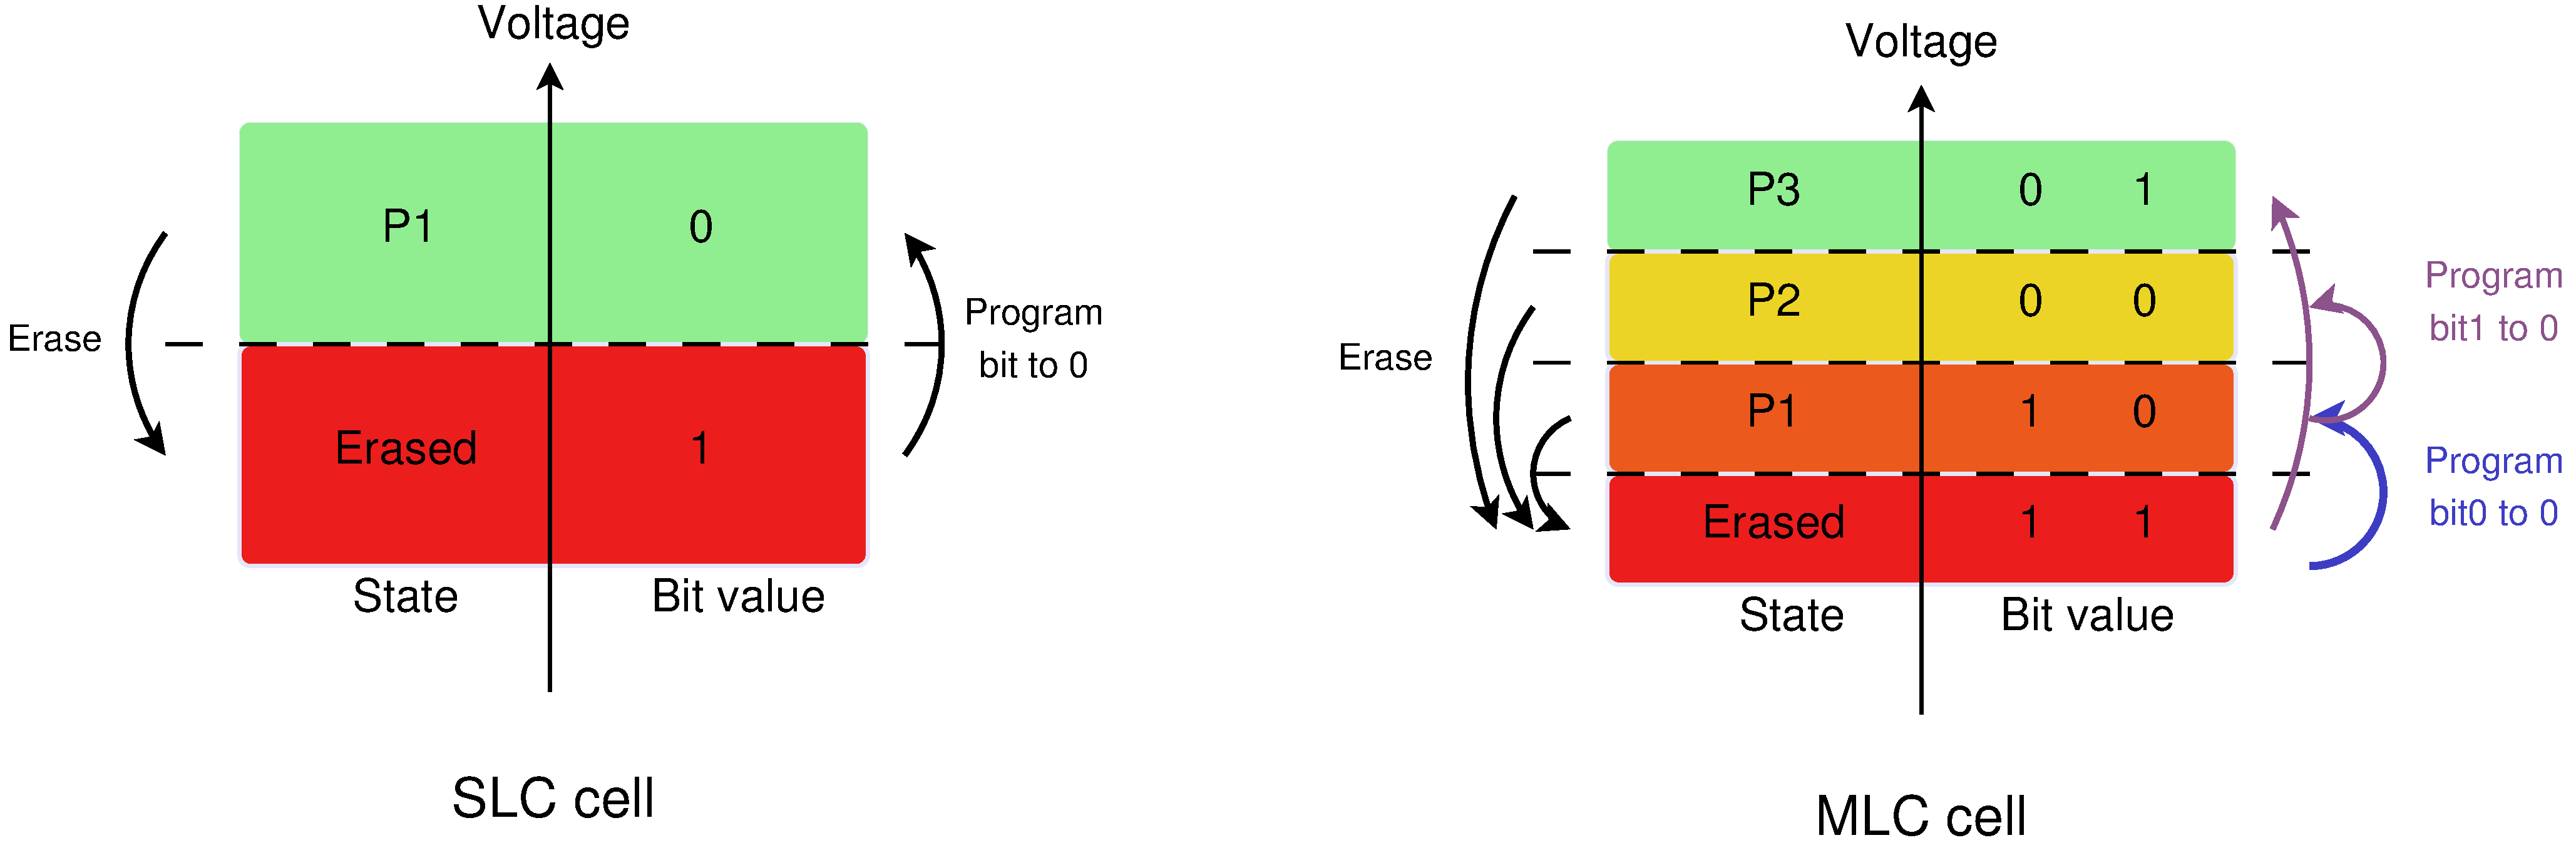
\includegraphics[scale=0.2]{slc-mlc-cell.pdf}
  \end{center}
\end{frame}

\begin{frame}{MLC NAND constraints: Paired pages}
  \begin{itemize}
  \item This is one of the biggest problem we have with MLC NANDs.
  \item MLC cells expose two bits.
  \item Each bit is assigned to a different page.
  \item Pages sharing the same cells are called "Paired pages".
  \item Paired pages are usually not contiguous.
  \item Pages have to be programmed in order.
  \item When programming the second page of a pair, you may corrupt
	the first page of the pair if the operation is interrupted.
  \end{itemize}
\end{frame}

\begin{frame}{MLC NAND constraints: Paired pages}
  \begin{center}
    \includegraphics[scale=0.5]{pairing-scheme.pdf}
  \end{center}
\end{frame}

\begin{frame}{MLC NAND constraints: What we discovered (bad news)}
  \begin{itemize}
  \item Modern MLC NANDs require data scrambling.
  \item Modern MLC NANDs show a high number of bitflips in the last
	set of programmed pages if the erase block is partially
	written.
  \item Both aspects seem to be related:
    \begin{itemize}
    \item NAND vendors try to mitigate the write-disturb effect by
	  accounting for future write-disturb when programming a page.
    \item These write-disturb prediction models are assuming random
	  data, hence the need for data scrambling/randomization.
    \end{itemize}
  \end{itemize}
\end{frame}

\begin{frame}{MLC NAND constraints: What we discovered (good news)}
  \begin{itemize}
  \item MLC NANDs can be programmed in 'SLC mode' (only write the first
	page of each pair)
    \begin{itemize}
    \item This solves the paired pages problem.
    \item Erase blocks written in 'SLC mode' show less bitflips.
    \item Erase blocks written in 'SLC mode' are less sensitive to
	  read/write disturbance.
    \end{itemize}
  \item To summarize, 'SLC mode' makes MLC NAND usable.
  \item But this also means exposing half the storage capacity.
  \end{itemize}
\end{frame}

\begin{frame}
  \begin{center}
  \Huge
  Questions? Suggestions? Comments?\\
  \vspace{1.5cm}
  \huge
  Boris Brezillon\\
  \large
  \vspace{0.5cm}
  \code{boris.brezillon@free-electrons.com}
  \vspace{0.5cm}
  \newline Slides under CC-BY-SA 3.0\\
  \scriptsize
  \url{http://free-electrons.com/pub/conferences/2016/elce/brezillon-ubi-mlc/}
  \end{center}
\end{frame}

\end{document}
